Seit der Entdeckung der kosmischen Höhenstrahlung 1912
von Victor Hess feiert die Astroteilchenphysik,
als junge Wissenschaft,
bahnbrechende Errungenschaften.
Mit der Entdeckung der Mikrowellenhintergrundstrahlung 1964,
gilt die Theorie des Urknalls
und eines expandierenden Universums als verifiziert.
Die moderne Astroteilchenphysik beschäftigt sich sowohl mit den
elementaren Bausteinen des Universums,
zum Beispiel durch die Suche nach Dunkler Materie,
als auch mit kosmischen Objekten
und den Beschleunigungsprozessen der emittierten Teilchen
und dessen Sekundärteilchen an sich.
Kosmische Botenteilchen liefern Informationen über
Aktive Galaxienkerne,
Neutronensterne
und weitere kosmische Phänomene,
wie zum Beispiel Supernovae und Gamma Ray Bursts.
Zu den wichtigsten kosmischen Botenteilchen gehören Photonen,
Protonen
und schwerere Kerne,
Neutrinos
und seit der ersten Detektion im Jahr 2015 werden Gravitationswellen als Boten
bezeichnet.
In diesem Versuch werden die Daten eines Detektors analysiert,
welcher für die Messung von hochenergetischer Gammastrahlung gebaut wurde.

% Seit der Entdeckung der kosmischen Höhenstrahlung
% 1912 von Victor Hess feiert die Astroteilchenphysik bahnbrechende Errungenschaften.
% Die Entdeckung der kosmischen Hintergrundstrahlung gilt als Beleg des
% expandierenden Universums und wirft dennoch weitere Fragen zum frühen Universum auf.
% Durch kosmische Botenteilchen ist das Erforschen von elementaren Bausteine und
% Beschleunigungsprozessen möglich.
% Anhand von kosmischen Botenteilchen können Informationen über Supernovae,
% Aktive Galaxienkerne und weitere kosmische Phänomene, wie zum Beispiel
% Neutronensterne und Gamma Ray Bursts, gewonnen werden.

\section*{MAGIC}%
\label{sec:magic}

\begin{wrapfigure}[13]{O}{0.45\textwidth}
		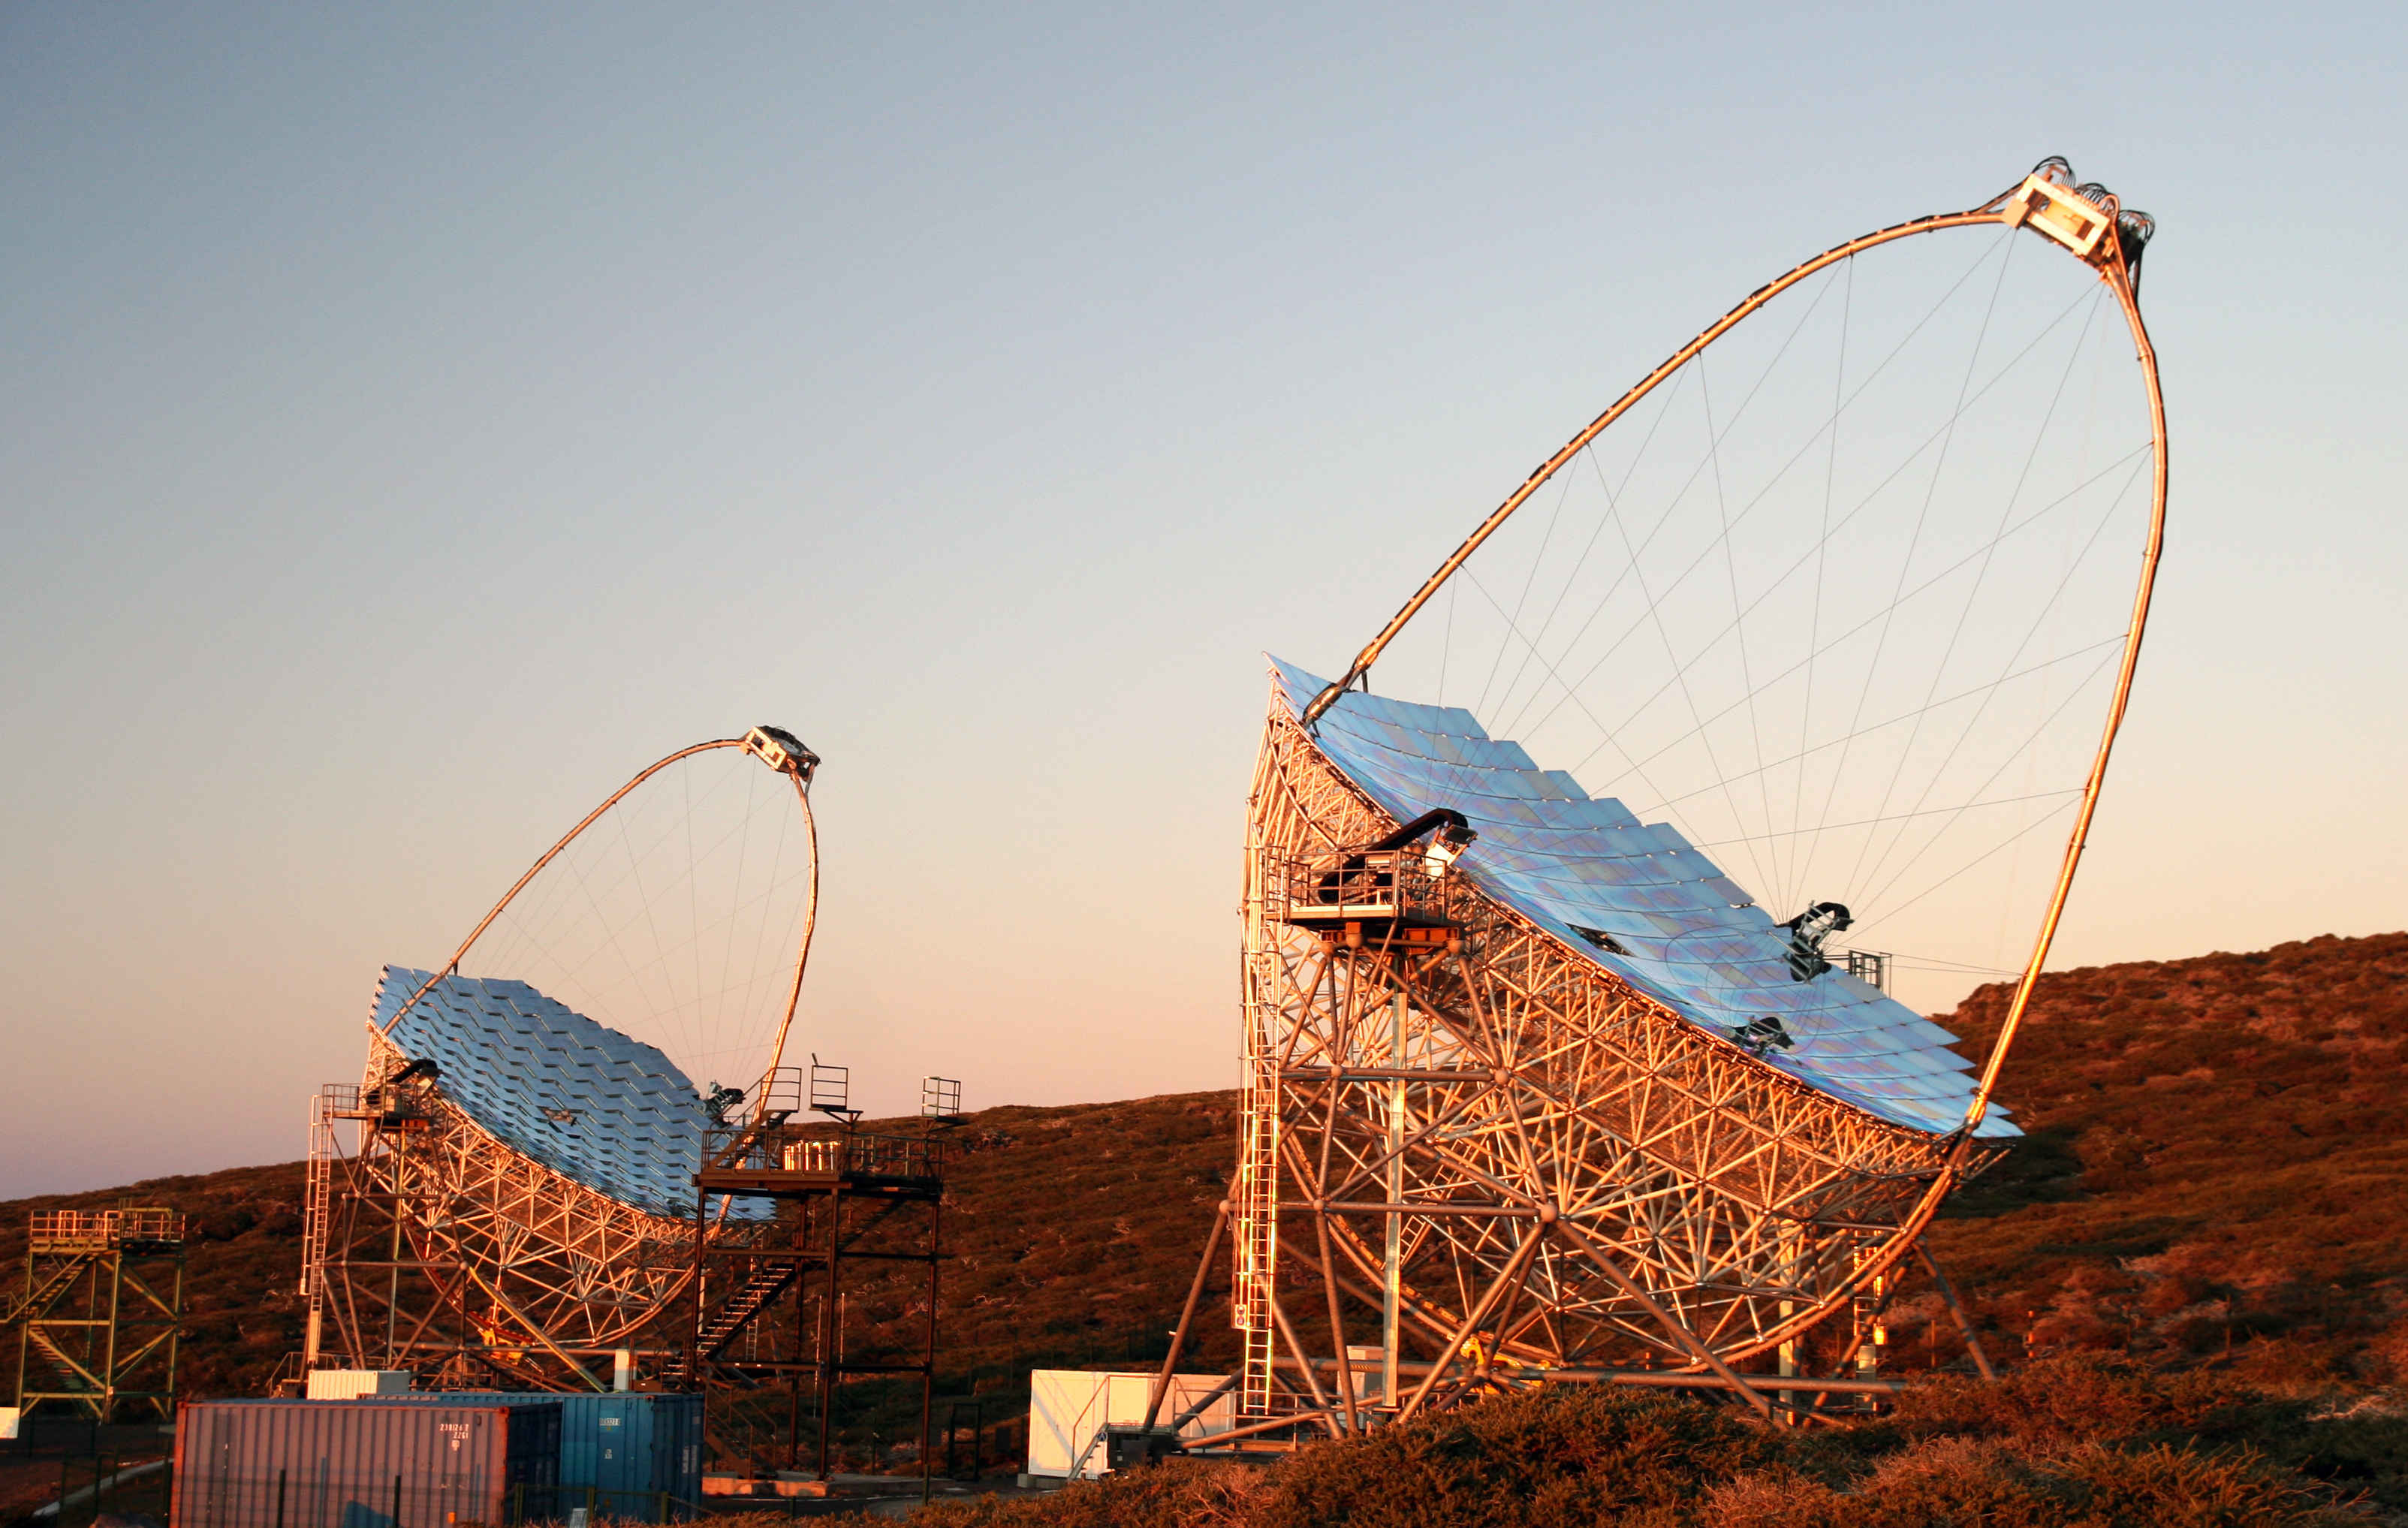
\includegraphics[width=\linewidth]{pictures/magic.JPG}
		\caption{MAGIC Teleskope in Observationsstellung.}%
		\label{fig:magic}
\end{wrapfigure}

% Bitte etwas uebersichtlicher strukturieren, zerst Teleskope, dann Gammas, dann Schauer und dann Tscherenkovlicht:
% Vorschlag:

% Einleitung ok, aber nicht auf Bild verweisen, erst spaeter.

Die \textbf{M}ajor \textbf{A}thmospheric \textbf{G}amma \textbf{I}maging
\textbf{C}herenkov Teleskope (Abbildung \ref{fig:magic}) sind derzeit das
weltweit größte im Stereomodus operierende IACT System.
MAGIC sucht nach Gamma Ray Bursts, beobachtet Blazare und untersucht das
Galaktische Zentrum.
Es befindet sich auf der kanarischen Insel La Palma auf dem Berg 'Roque de Los Muchachos',
in einer Höhe von 2200m über dem Meeresspiegel.
Es ist für Gammastrahlung in einem Energiebereich von
\SI{50}{\giga\electronvolt} bis \SI{50}{\tera\electronvolt} sensitiv.
Beide Teleskope haben eine Spiegelfläche von je \SI{17}{\meter} Durchmesser,
welche die Schauerbilder auf eine Kamera aus 1039 Photo Multiplier Tubes (PMTs) abbilden.
Der Detektor besitzt ein Sichtfeld von \SI{3,5}{\degree}.

\begin{wrapfigure}[13]{I}{0.45\textwidth}
		\includegraphics[width=\linewidth]{tikz/build/shower.pdf}
		\caption{Teilchen in einem Teilchenschauer mit einem Photon als
    Pri\-mär\-teil\-chen.}%
    \label{fig:schauer}
\end{wrapfigure}
Treten hochenergetische Gammateilchen in die Erdatmosphäre ein,
wechselwirken sie mit den darin enthaltenen Atomkernen
und produzieren durch Paarerzeugung relativistische Elektronen
und Positronen.
Durch Bremsstrahlung werden wiederum relativistische Photonen erzeugt.
Durch das Wechselwirken (Paarerzeugung und Bremsstrahlung) weiterer
Sekundärteilchen entsteht ein Schauer aus Photonen und Leptonen (Abbildung
\ref{fig:schauer}).
Da die geladenen Teilchen im Schauer relativistische Geschwindigkeiten besitzen,
strahlen diese bei der Propagation durch die Atmosphäre Tscherenkowlicht ab.
Ein durch ein in die Erdatmosphäre eintretendes Gammateilchen ausgelöster
Tscherenkowblitz dauert nur einige Nanosekunden
und ist somit mit dem menschlichen Auge nicht erfassbar.

% Der Nachweis von hochenergetischer Gammastrahlung ist auf der Erde aufgrund der
% Atmosphäre nur indirekt möglich.
% Hochenergetische Photonen und Hadronen
% wechselwirken beim Eintritt in die Erdatmosphäre mit dieser
% und erzeugen sogenannte Teilchenschauer,
% eine Kaskade aus wiederum wechselwirkenden Teilchen.
% Aufgrund ihrer relativistischen Geschwindigkeiten
% strahlen geladene Schauerteilchen Tscherenkowlicht ab,
% welches auf der Erde von sehr sensitiven Teleskopen,
% sogenannten IACTs (Imaging Air Cherenkov Telescopes)
% gemessen werden kann.
% erzeugen in der Atmosphäre
% Teilchenschauer (siehe Abbildung~\ref{fig:schauer}), die aufgrund ihrer relativistischen Geschwindigkeiten Tscherenkowlicht abstrahlen.
% \begin{wrapfigure}[13]{I}{0.45\textwidth}
% 		\includegraphics[width=\linewidth]{tikz/build/shower.pdf}
% 		\caption{Teilchen in einem Teilchenschauer mit einem Photon als
%     Pri\-mär\-teil\-chen.}%
%     \label{fig:schauer}
% \end{wrapfigure}
% MAGIC ist derzeit das größte Stereoteleskop,
% welches in einem Energiebereich von \SI{50}{\giga\electronvolt} bis
% \SI{50}{\tera\electronvolt} sensitiv ist.
% Es steht auf der Insel La Palma auf einer Höhe von \SI{2200}{\meter}.
% Propagiert ein geladenes Teilchen mit einer Geschwindigkeit in einem
% Medium, die höher als die Lichtgeschwindigkeit in diesem Medium ist,
% so erzeugt dieses Tscherenkow-Photonen.
% Die ultrarelativistischen Photonen, welche in die Erdatmosphäre eintreten,
% wechselwirken mit den darin enthaltenen Teilchen beispielsweise über
% Bremsstrahlung oder Paarerzeugung und produzieren somit weitere
% relativistische Teilchen, welche wiederum Tscherenkowkegel erzeugen.
% Dabei partitioniert das Primärteilchen die Energie solange, bis die Energie
% nicht mehr ausreicht Sekundärteilchen zu produzieren.

% Die dadurch erzeugten Lichtblitze können durch Tscherenkowteleskope gemessen
% werden.
% Die Spiegelfläche von \SI{17}{\meter} Durchmesser besteht aus \num{974} einzelnen
% Spiegeln, die auf \num{1039} Photo Multiplier Tubes (PMTs) abbilden.
% Das Teleskop besitzt ein Field of View von \SI{3.5}{\degree}.

% Ziel ist es, mit den Teleskopen Gamma-Quellen wie AGNs, Supernovae und
% Gasverteilungen, in denen viel Sternbildung stattfindet, zu observieren, um etwas
% über die fundamentalen physikalischen Prozessen in der Quellregion zu erfahren.
% Aufgrund der hohen Energien die bei stellaren Prozessen erzeugt werden, können
% so Effekte auf Energieskalen beobachtet werden, welche nicht mit irdischen
% Teilchenbeschleunigern erzeugt werden können.
% Des Weiteren wird nach einen indirekten Nachweis nach dunkler Materie gesucht.
% Fundamentales Problem ist, dass geladene Teilchen jegliche Richtungsinformation
% in kosmologischen Magnetfeldern verlieren und somit keine Informationen zur
% Quelle rekonstruiert werden kann.
Neben hochenergetischen Photonen lösen auch kosmische Protonen,
beim Eintritt in die Erdatmosphäre Teilchenschauer aus.
Obwohl sich die Zusammensetzung dieser stark von der von Gammaschauern unterscheidet,
entstehen letztendlich durch leptonische Komponenten in den hadronischen Schauern Tscherenkowblitze,
die den gesuchten Blitzen sehr ähnlich sehen.
Eine der großen Herausforderungen einer Analyse von IACT Daten liegt in der Unterscheidung von elektromagnetischen (Signal) und  hadronischen (Untergrund) Schauern.
Ziel des Verusches ist es ein Überblick über die Funktionsweise 
und die Datenanalyse von Abbildenden Cherenkov-Teleskopen, 
sowie die Interpretation von experimentellen Daten 
der Astroteilchenphysik vermittelt.
% \textit{Die etablierte Methode zur Signal-Untergrund-Trennung ist in dieser Analyse das
% Machine Learning. (Dies ist Schwerpunkt des Lehrstuhlversuches Analyse von FACT-Daten \cite{fact}.)
% Ziel dieses Versuches ist die Durchführung einer Analysekette, um von
% kalibrierten Daten zu physikalischen Parametern von astrophysikalischen Quellen
% zu gelangen.}

\section*{Krebsnebel}%
\label{sec:krebsnebel}

\begin{wrapfigure}{O}{0.35\textwidth}
		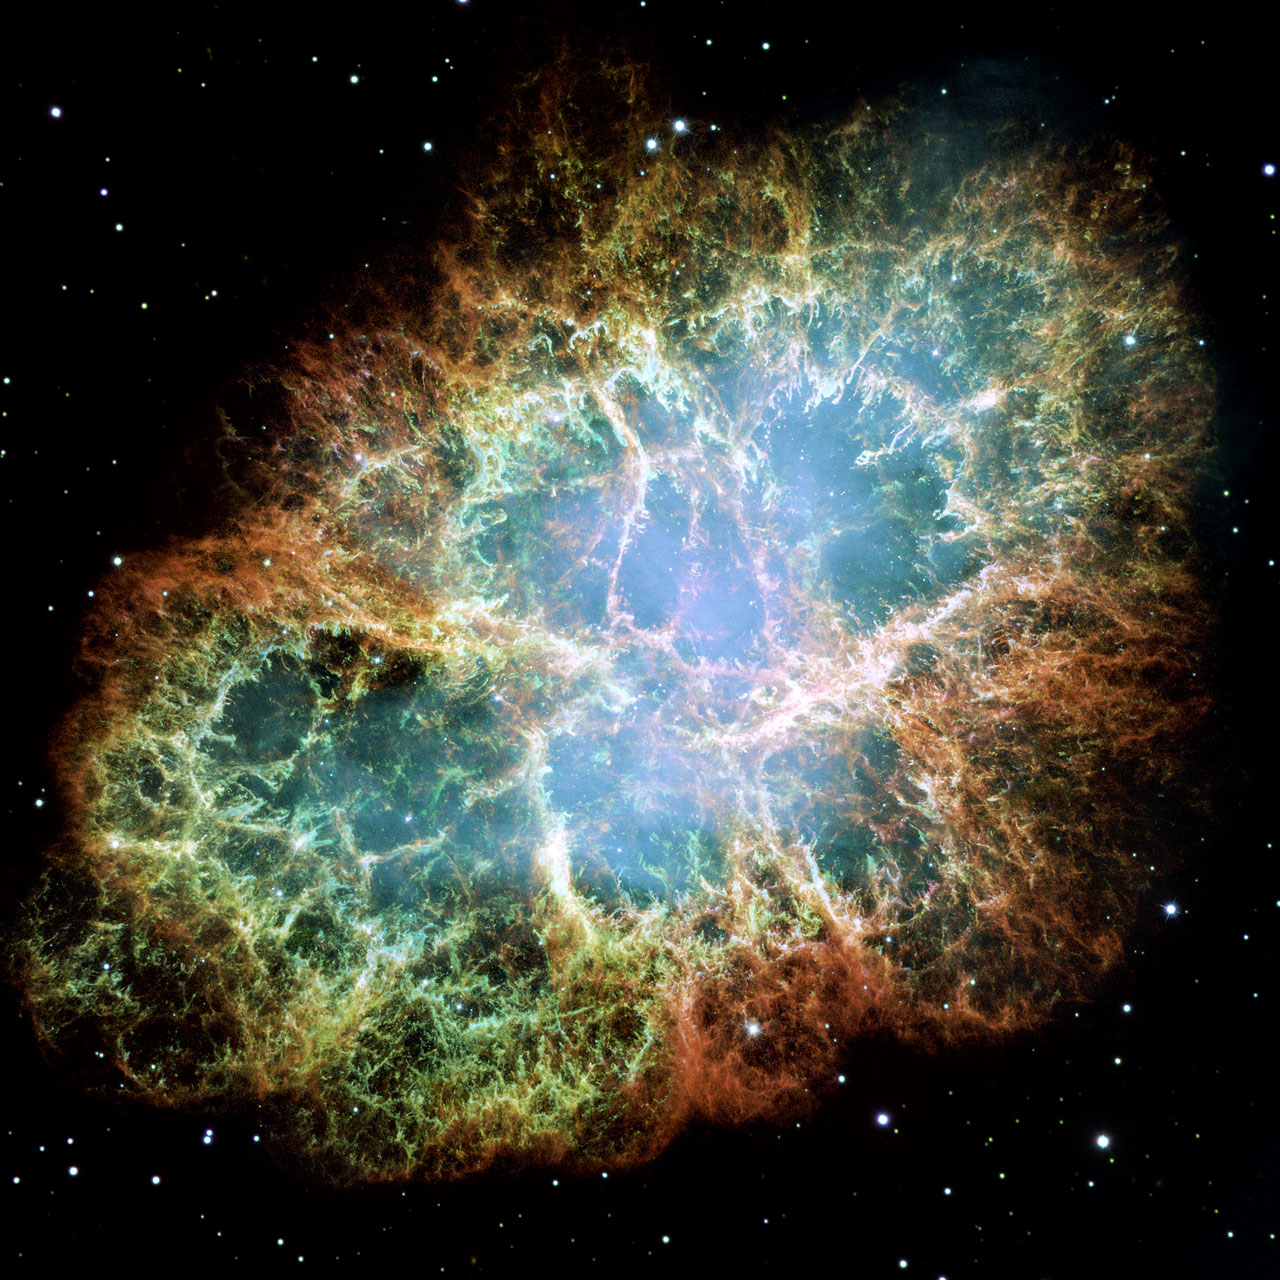
\includegraphics[width=\linewidth]{pictures/crab.jpg}
		\caption{Krebsnebel aufgenommen mit dem Hubble Teleskop.}%
    \label{fig:crab}
\end{wrapfigure}

In diesem Versuch wird der Krebsnebel untersucht.
Er ist ein Überrest einer Supernova-Explosion eines Sterns
mit 8~bis 12 Sonnenmassen beobachtet im Jahr 1054,
und befindet sich im Sternbild Stier.

Eine Supernova-Explosion ist das Ende eines massereichen Sterns,
bei der die Leuchtkraft eines Sterns kurzzeitig auf das millonen- bis
milliardenfache der ursprünglichen Leuchtkraft ansteigt,
ehe der Stern nach dem Verbrauch des
nuklearen Brennstoffs kollabiert und ein kompaktes Objekt
(Neutronenstern oder Schwarzes Loch) bildet.

Im Zentrum des Krebsnebels befindet sich ein Pulsar,
welcher die Quelle von starker elektromagnetischer Strahlung ist.
Pulsare sind schnell rotierende Neutronensterne,
welche sehr regelmäßige, kurze Pulse emittieren.
Typische Größen von Neutronensternen sind Durchmesser von einigen
\SI{10}{\kilo\meter}.
Die Materiereste, die bei einer Supernova-Explosion
vom zurückbleibenden Neutronenstern abgesprengt werden,
bilden eine überschallschnelle Schockwelle.
Diese heizt bei der Expansion das interstellare Medium auf Temperaturen von bis zu
\SI{e8}{\kelvin} auf.
Die propagierenden Schockwellen können durch Dichteschwankungen des stellaren
Mediums Sternbildung auslösen
und sind außerdem Lieferant für schwere Elemente, die in einem normalen
Fusionsprozess eines Sterns nicht gebildet werden können.
Der zurückbleibende Neutronenstern besitzt ein intensives Magnetfeld,
in dem hochenergetische Elektronen Synchrotonstrahlung erzeugen.
Des Weiteren kommt es zur Invers-Compton-Streuung,
bei dem ein hochenergetisches Elektron einen Teil seiner
Energie auf ein Photon überträgt.
Niederenergetische Photonen werden durch thermische Strahlung produziert.
MAGIC detektiert Photonen,
die aus der Materie,
die bei der Supernovae abgestoßen wird,
emittiert werden.
Durch mehrfache Streuung und Synchrotonstrahlung entstehen so hochenergetische Gammateilchen,
die MAGIC detektieren kann.

Aufgrund seiner Eigenschaften wird er als Standardkerze der Gamma-Astronomie betitelt,
da der Teilchenfluss hier nahezu konstant und aufgrund der Nähe der Quelle vergleichsweise hoch ist.
% Durch seine Analyse kann die Performance von verschiedenen Teleskopen verglichen werden.
Mit Messdaten des Krebsnebels können unter Anderem Analysemethoden geprüft
oder die Performance verschiedener Detektoren verglichen werden.

\subsection*{Detektion}%
\label{sub:wobbelmodus}

% Da kosmische Quellen nicht isoliert von ihrer Umgebung betrachtet
% werden können,
% müssen zu jeder anvisierten Quellposition Umgebungsdaten aufgenommen werden.
% Die
% % wird zu jeder
% Quellposition heißt \textit{On}.
% % genau so lang Daten aufgenommen,
% % wie
% % und die
% Positionen nahe der Quellposition,
% in denen kein Gammafluss erwartet wird,
% heißen \textit{Off}.


Obwohl bei der Signal-Untergrund-Trennung ein großer Teil der hadronische Schauer aussortiert werden kann, bleibt
dennoch ein gewisser Anteil an Untergrund Ereignissen bestehen.
Da von einem
isotropen hadronischen Untergrund
innerhalb des Blickfeldes von MAGIC
ausgegangen werden kann,
ist eine Messung des Untergrundes an
einer äquivalenten Position ohne signifikante Gammaquelle möglich.
Somit kann
% in der Analyse der Untergrund von der Messung abgezogen werden, sodass nur das
in der Analyse ein Modell des Untergrundes an der Quellposition aus den
Messungen der Untergrundpositionen erstellt werden.
Ereignisse aus der Quellposition,
die dem Untergrundmodell ähnlich sehen, werden verworfen,
sodass nur noch das Signal (Exzess) übrig bleibt.
% Durch das Modell kann damit der Untergrund in der Quellposition zu minimiert werden,
% sodass nur das Signal (der Exzess) uebrigbleibt.
Die Quellposition heißt \textit{On}-Position, äquivalente Positionen ohne
Gammaquelle heißen \textit{Off}-Position.
Eine Möglichkeit wäre nun zwei Messungen durchzuführen: eine für die
Signalmessung an der On-Position und eine Untergrundmessung an einer
nahegelegenen Off-Position.


% Die Teleskope triggern drei Arten von Events.
% Neben den eigentlichen Luftschauern,
% welche durch Protonen
% oder Gammas verursacht werden,
% erzeugen Myonen oder versehentliche Trigger weitere Events.
% Myonen erzeugen ringförmige Ereignisse in der Kamera.
% Versehentliche Trigger entstehen z.B.\ durch den Nachthimmelhintergrund
% (\textit{Night Sky Background, NSB}) und elektronisches Rauschen.

% In der Gamma Ray Astronomie werden die Teleskope in der Regel auf einen Punkt
% ausgerichtet, an dem eine Quelle angenommen wird.
% Die gemessenen Events, die das Teleskop triggert, können vom
% kosmischen Hintergrund oder von einer echten Quelle, falls diese existiert, sein.

MAGIC nimmt Daten im Wobble-Modus auf.
Die erwartete Quellposition liegt dabei nicht im
Kameramittelpunkt,
sondern um
\SI{0.4}{\degree} um den Kameramittelpunkt
verschoben.
In äquidistanten Abständen um den Kameramittelpunkt
werden Off-Positionen bestimmt (siehe Abbildung~\ref{fig:hillas}).
Dies hat den Vorteil, dass die Aufnahme von On und Off Daten zeitgleich möglich
ist und so die Messzeit maximiert wird.

% Anschließend wird der Abstand $\theta$ der rekonstruierten
% zu der On- und den Off-Positionen bestimmt.
% Die Bins von $\theta^2$ werden in den Off-Positionen
% anhand der On-Position (Anzahl Off-Positionen / Messzeiten) normiert.
% Im Anschluss wird der aus den Off-Positionen bestimmte Untergrund
% aus der Messung der On-Position subtrahiert, sodass Signal übrig bleibt
% (vgl. Abbildung~\ref{fig:thetacut}).

\clearpage
